\chapter{Constraints}\index{constraints|textbf}\label{Chap:constraints}

From the perspective of information theory, it is not straightforward to categorize the amount of structural information in a powder diffraction pattern. From one perspective, every reflection that is within the measured data range does provide some information about the positions and ADPs for the atoms, even if it does not have intensity above the background level, but this information is compromised by the overlap of reflections. Since background levels are higher in powder diffraction than single-crystal diffraction (since single-crystal background is spread over $4\pi$ steradians in volume while powder background is only spread in one dimension, so there will be a higher uncertainty about when a reflection intensity is small. In single-crystal diffraction, the number of observations tends to scale with the complexity of the structure, but that is not always the case with powder diffraction. The resolution and sensitivity of the instrument, as well as sample broadening effects limit the amount of information that can be measured with powders. Further, static and dynamic disorder can reduce the range where diffraction can be observed, so complex structures may provide data over a narrower range of Q than a simple structure, as much as we might wish otherwise. 

With more complex structural models, one may not have enough well-determined independent observations to fit all independent parameters that are available. Better data may help this by separating more reflections or by improving signal-to-noise allowing one to see more weak peaks. Likewise, there are sometimes parameters that cannot be differentiated regardless of the data type. As an example of the former, for x-ray diffraction from a complex metal oxide, the ADP values for the O atoms, where each will have a minor impact on the overall scattering, may refine to pretty much random values. This is where constraints can help. 

What constraints are is a way to reduce the complexity of a model by designating that parameters are linked together is some way. As an example, we can indicate that all O atoms in a model have the same $\rm U_{iso}$ value, so if we have 10 O atoms, rather than having 10 $\rm U_{iso}$ values, we now have a single parameter that dictates the $\rm U_{iso}$ for all 10 atoms. A constraint can also be an equation. If we create a constraint that $\rm Occ_1 + Occ_2 = 1$, where $\rm Occ_j$ is the occupancy for atom $j$, then what we are doing is to create a new parameter, which we can call $\delta_{occ12}$ and rather than varying the two parameters $\rm Occ_1$ and $\rm Occ_2$ we vary $\delta_{occ12}$ where the occupancies become $\rm Occ_1-\delta_{occ12}$ and $\rm Occ_2+\delta_{occ12}$. 

Thus, in our complex metal oxide that we discussed above, where individual $\rm U_{iso}$ values for O have a small leverage on the overall fit, what is commonly done is to introduce a constraint that all O atoms will share the same $\rm U_{iso}$ value. This will increase how much impact the $\rm U_{iso}$ value has on the quality of the fit, ensuring that a more accurate value is more likely and at the same time it decreases the complexity of the model. As an example for the case where parameters cannot be distinguished, consider a site that is shared by two different types of atoms. Since the coordinates or $\rm U_{iso}$ value for each of these two atoms will contribute in exactly the same manner to every $F_{hkl}$ value, changing will have the same effect as changing the other. The x, y and z fractional coordinates and $\rm U_{iso}$ value for the two atoms sharing a site must be constrained to be the same. 

Constraints are implemented in GSAS-II by summing the derivatives for all constrained parameters to determine the effect of changing the now grouped parameters and then when a shift is computed, all grouped parameters are set to the same value. Atom coordinates are handled slightly differently, in that shifts are applied to atom positions, but the effect is the same.

One special case of constraints are those of rigid bodies, where the geometry for a group of atoms that are refined together will be defined. Rigid bodies are sufficiently complex that they are described in a separate chapter, \ref{Chap:rigidbody} and are implemented in another manner than what is described here. 

\section{GSAS-II Parameter Naming}\label{ref:paramname}

Every parameter that can be refined in GSAS-II is defined a unique name that is associated with a value. These names are referenced when defining constraints and restraints. The naming follows this convention: 
\begin{quote}
 \textbf{P}:\textbf{H}:\textbf{name}    
\end{quote}
where \textbf{P} is a phase number and \textbf{H} is a histogram number and \textbf{name} specifies the type of parameter. The \textbf{name} values are tabulated in the GSAS-II Developer's Documentation in the table at this URL: \url{https://gsas-ii.readthedocs.io/en/latest/objvarorg.html\#parameter-names-in-gsas-ii}.
When not appropriate, \textbf{H} or \textbf{P} can be blank. Global parameters, which are very uncommon, do not have an \textbf{H} or \textbf{P} value. Note that internally to GSAS-II, parameter names are stored in a fashion that abstracts the phase and histogram numbers, so that if the phases or histograms are reordered, the names will automatically be updated to follow. 

As an example of how a number would be omitted, a wavelength is a parameter of a histogram and not a phase and the name LAM is associated with wavelength. Thus, the wavelength for histogram 3 will be named \texttt{:3:LAM} . 

Atom parameters are named with an additional number (note that the histogram number is omitted as atoms are not associated with phases:
\begin{quote}
    \textbf{P}::\textbf{name}:\textbf{atom-num}
\end{quote}
As an example of that, \texttt{1:Uiso:12} is the $\rm U_{iso}$ value for atom 12 in phase 1. Note one complication for atom coordinates. While atom coordinates parameter names for atom \texttt{n} in phase \texttt{p} are \texttt{p:Ax:n}, \texttt{p:Ay:n}, and \texttt{p:Az:n},  the parameters that are varied are named  \texttt{p:dAx:n}, \texttt{p:dAy:n}, and \texttt{p:dAz:n}. These ``dA*'' values are offsets that are applied to coordinates rather than the coordinates themselves. In this way when an atom is at a site x,1/2-x,z only the change, $\delta$x is computed and is added to the x coordinate and subtracted from the y coordinate. 

Finally, as noted in \S\ref{ref:HAP}, the HAP parameters have values for each phase and each histogram. As an example there can be March-Dollase texture parameter for every phase and every histogram and it will be named \texttt{1:2:MD} for phase 1 and histogram 2. 

Alas, there is one place where this naming is confusing, but a change would likley introduce bugs that we would need to spend years finding and fixing. Every histogram has a scale factor, named \texttt{:0:Scale} (etc.), but there are HAP parameters for phase fractions and these use the same name, \texttt{0:0:Scale} (etc.). They are distinguished by the scale factor having no phase number while the phase fraction has both. 

\section{GSAS-II Constraint Types}

In GSAS-II constraints are created, viewed or changed from the constraints data tree entry. For the purposes of simplification, constraints are broken into five categories with matching data tabs: Phase constraints, Histogram constraints, HAP constraints (labeled Histogram/Phase), Global constraints (usually not used) and Sym-Generated constraints. The latter tab shows any constraints that are generated by symmetry on lattice or atom parameters (such as one that enforces $a=b$ for a tetragonal cell or $x=y=z$ for an atom at a $x,x,x$ special position). These Sym-Generated constraints are read-only. 

After selecting a tab, one will see a display of existing constraints, which can be deleted or their coefficients can be edited. If a constraint is specified for a set of parameters where none of the parameter are varied, the parameter is not used, but it is noted here that the parameter exists, but is being ignored. If some parameters, but not all are varied in constraint, that can generate an error. Likewise, a message is generated if constraints are in conflict. Constraints are created using the commands in the ``Edit Constr.'' menu, but one must select the type of constraint to be varied. 

There are four types of GSAS-II constraint entries:

\subsection{Parameter equivalences:}
Parameter equivalences can be thought of as where one or more parameters are set from a controlling parameter. This can be written in the form:
$$var_C \rightarrow  c_1 var _1 = c_2 * var_2 = ...$$
where $c_j$ are constants and $var_j$ are the names of a GSAS-II parameters, named \textbf{P}:\textbf{H}:\textbf{name}. Of the parameters, $var_C$ is the controlling parameter and the others are set from this. 

As an example for the use of a parameter equivalence, suppose I want to constrain all four of the O atoms in my phase to be varied as a single parameter. I use the ``Edit Constr.''/``Add equivalence'' menu command and the first window that is displayed after the menu command, as seen in Fig. \ref{fig:equiv1}, will show all the parameters for the selected tab (Phase, Histogram, HAP). I can pick a Uiso parameter for any of the O atoms in that window. The window in Fig. \ref{fig:equiv2} is shown next.  Here, I select a ``wildcard'' parameter for all O atoms in this phase.  
\begin{figure}
    \centering
    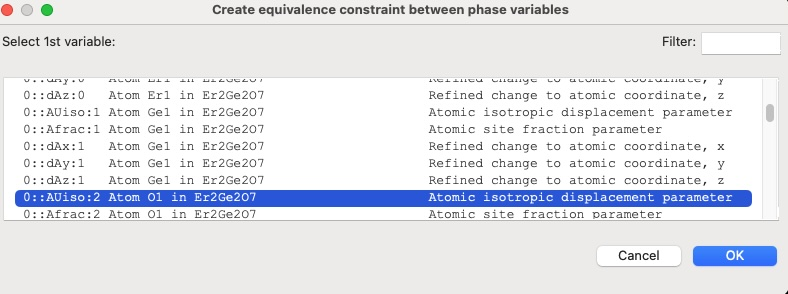
\includegraphics[width=0.75\linewidth]{figures/Equiv1.jpg}
    \caption{First window when creating a parameter equivalence.}
    \label{fig:equiv1}
\end{figure}
\begin{figure}
    \centering
    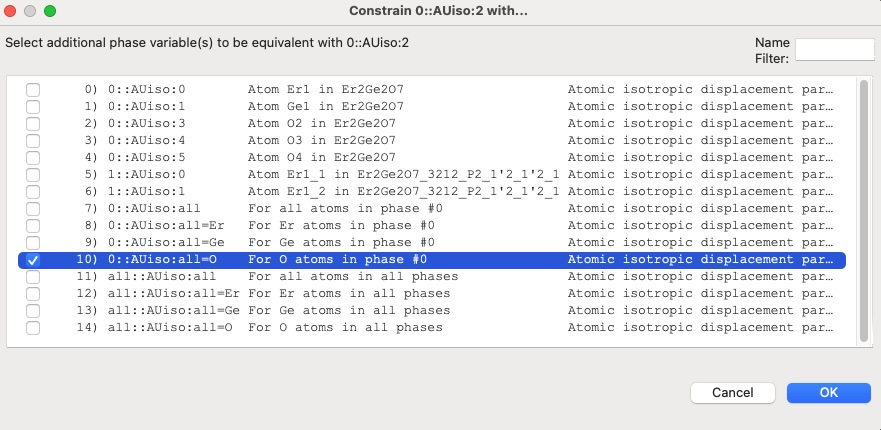
\includegraphics[width=0.85\linewidth]{figures/Equiv2.jpg}
    \caption{Second window when creating a parameter equivalence.}
    \label{fig:equiv2}
\end{figure}
When this is done, a warning window is commonly shown such as the one in Fig. \ref{fig:equiv3}. This warning is shown when a constraint involves parameters that are not varied. The constraint will be ignored. If you went to the bother of creating the constraint, you likely want to use it, so the warning is to tell you that you now need to set the refine flags for the Uiso parameters. Provided that you press ``Yes'' on this window, the equivalence will now appear on the constraints data window, as seen in Fig. \ref{fig:equiv4}. Should you wish to change the ratios applied in the equivalence (the $c_j$ values), you would press the ``Edit'' button next to the constraint. 
\begin{figure}
    \centering
    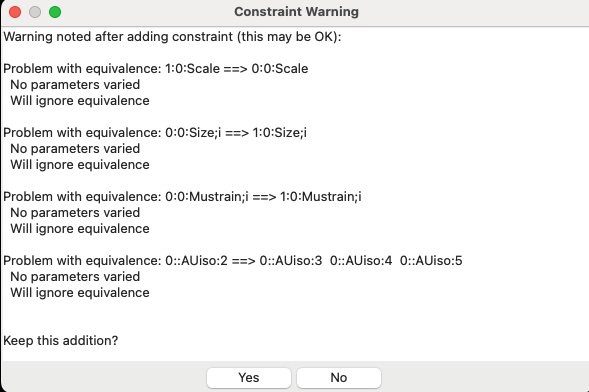
\includegraphics[width=0.5\linewidth]{figures/Equiv3.jpg}
    \caption{Warning that a constraint has been created for unvaried atoms. This is normal.}
    \label{fig:equiv3}
\end{figure}

\begin{figure}
    \centering
    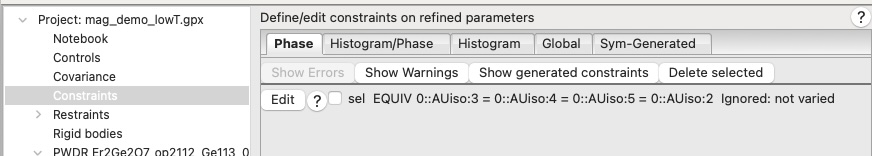
\includegraphics[width=0.75\linewidth]{figures/Equiv4.jpg}
    \caption{The data window showing the newly Enter Caption}
    \label{fig:equiv4}
\end{figure}
\subsection{Constraint equations:}
Constraint equations are written in the form:
$$c_1 var _1+ c_2 * var_2 + ... = T$$
where $c_j$ and $T$ are constants and $var_j$ are the names of a GSAS-II parameters, named \textbf{P}:\textbf{H}:\textbf{name}. There is no limit to the number of variables that can be included in a constraint equation. 

Use the ``Edit Constr.''/``Add constraint equation'' menu command to create a new constraint equation. 
The first window that is displayed after the menu command, as seen in Fig. \ref{fig:constr1}, will show all the parameters for the selected tab (Phase, Histogram, HAP) and after a parameter is selected. 
In the figure I have used a filter to select only fractional occupancies by requiring the string ``frac'' to be present. 
In Fig. \ref{fig:constr2} , the next window that is opened is shown. Note that this window only shows parameters that are related to the first parameter (here type ``Afrac'') , where you can select all the parameters you wish to constrain. 
Note that at the end of that list, you can select ``wildcard'' parameters, which will select all the matching parameters with any histogram and/or phase number. After OK is selected on the second window, the constraint is created. 
When a constraint equation is created, the $c_j$ and $T$ values are initially set to 1, but using the ``Edit'' button next to the constraint on the data window for the Constraints data tree entry allows those values to be edited. 
\begin{figure}
    \centering
    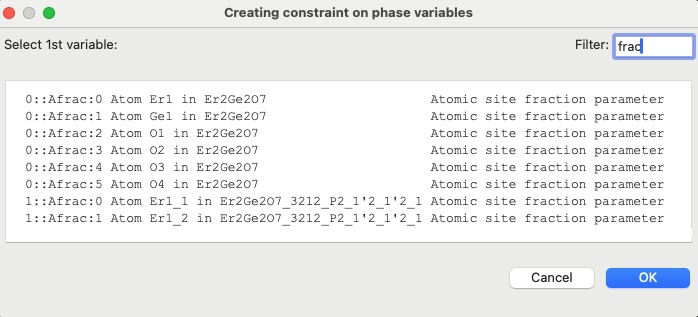
\includegraphics[width=0.75\linewidth]{figures/ConstrVar1.jpg}
    \caption{First window when creating a constraint equation.}
    \label{fig:constr1}
\end{figure}
\begin{figure}
    \centering
    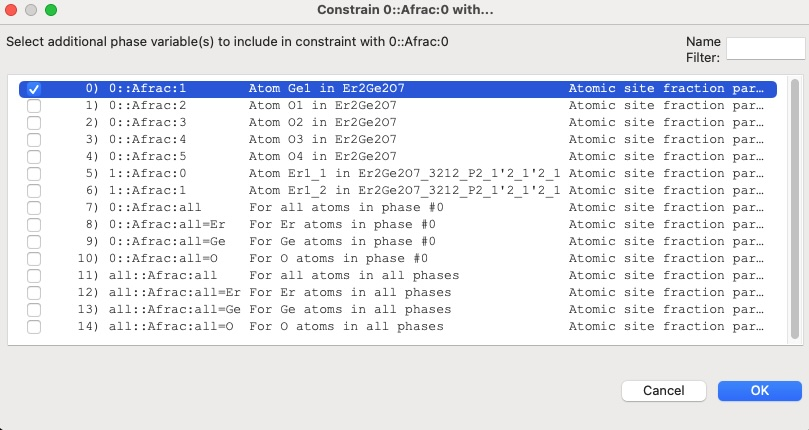
\includegraphics[width=0.75\linewidth]{figures/ConstrVar2.jpg}
    \caption{Second window when creating a constraint equation.}
    \label{fig:constr2}
\end{figure}
You may notice that the parameter equivalence that was initially presented, 
$$var_C \rightarrow  c_1 var _1 = c_2 * var_2 = ...$$
is no different than a series of constraint equations: 
\begin{align}
    var_C&  - c_1 var _1 &= 0\\
    var_C&  - c_2 var _2 &= 0\\
    var_C&  - ... &= 0
\end{align}
Why are both options available? It is much simpler to set up and understand parameter equivalences than a series of constraint equations. Also the implementation for equivalences is a bit simpler. So, both are offered in GSAS-II. Under special circumstances GSAS-II will convert parameter equivalences to constraint equations as described below in \S\ref{ref:constraintcalc}.

\subsection{New Variable definitions:}\label{ref:newvar}
New variable definitions are used to establish parameters that group parameters in alternate ways. They are not commonly created by users, but an example for how they might be used follows. Suppose we have two very closely coupled parameters, say for two atoms that are related by a pseudo-mirror plane, so that the x and y coordinates for each atom are highly correlated with each other. If the two x coordinates are \texttt{p:dAx:1} and \texttt{p:dAx:2} and we define two new variables:

$$ \texttt{p:dAx:1} + \texttt{p:dAx:2} = \rm Xsum12$$
$$ \texttt{p:dAx:1} - \texttt{p:dAx:2} = \rm Xdif12$$
Now, if we refine $\rm Xsum12$ and do not refine $\rm Xdif12$ then the two atoms will move together. In the final stages of the fit, we can see if the data have enough sensitivity to the differences between the impact of two atoms on the model by testing to see if fitting $\rm Xdif12$ is possible. 

The process of creating a new variable in the GSAS-II GUI is largely the same as creating a constraint equation, except that the ``Edit Constr.''/``Add New Var'' menu command is used. The windows that follow are almost identical to those in in Fig. \ref{fig:constr2} and in Fig. \ref{fig:constr2}.  

One major role for new variable constraints is to implement refinement of representational analysis distortion modes. This will be discussed in \S\ref{ref:RA}. These are typically created by reading in a CIF created on the ISODISTORT web site. 

\subsection{Parameter holds:}
Parameter holds are used to prevent a parameter from being fit. These are typically used where a single refine flag will set several parameters to be refined, but one of those parameters should not be fit. These are not commonly needed. 

An example where a parameter hold would be used would be with a structure in a polar space group. As was described in \S\ref{ref:polar}, one or more coordinates must be fixed. In the example used in \S\ref{ref:polar},  with space group $P 2_1$, the origin for the $b$ axis is undefined. One likely want to vary all the atom coordinates except one of the y values. Fixing a ``dAy'' parameter for one atom will prevent that one variable from being refined. 

Set the parameter hold by selecting the ``Edit Constr.''/``Add hold'' menu command. A window will be opened where parameter(s) can be selected. In Fig. \ref{fig:Hold} this window is shown. Note that a parameter named ``Ay'' will be the variable name for an atomic y coordinate, so that string has been used to search for atom y coordinate variables. Selecting any of the listed variables will fix one atom's y coordinate. 

\begin{figure}
    \centering
    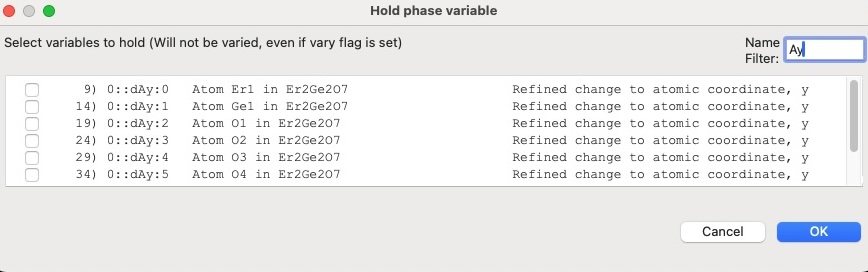
\includegraphics[width=0.8\linewidth]{figures/HoldVar.jpg}
    \caption{Selecting a parameter to hold. Note use of filter to reduce the number of displayed options.}
    \label{fig:Hold}
\end{figure}

\subsection{Make Atoms Equivalent}
The ``Edit Constr.''/``Make Atoms Equivalent'' menu command is a shortcut that will perform the several commands needed to treat atoms that share a site. After using this, one selects two (or more) atoms that share a site. Parameter equivalences will be created for the x, y, z, and Uiso parameters for the selected atoms, and a constraint equation will be created that forces the sum of the atom occupancies to be 1. The result is no different than if the individual parameter equivalences and constraint equation had been done in five separate steps. 

\section{Constraint and New Variable Processing}\label{ref:constraintcalc}
The processing of constraint equations and new variable equations requires some abstract linear algebra since a parameter may show up in more than one equation. The equations are collected into groups where each parameter is referenced in only one group. If there are $n$ parameters in the group, then there must be $n$ or fewer equations. If there are $n$ equations, then the constraints uniquely determine the values of all parameters. If there are more than $n$ equations then the constraints are either overdetermined or a constraint is duplicated in some fashion; either case is treated as an error. If there are $m$ equations ($m < n$) then there are still $n-m$ remaining degrees of freedom. The remaining degrees of freedom are computed as to be as best orthogonal from the $m$ equations and these specify the variables that can be refined. Effectively what is done is that new variable equations are generated for the remaining degrees of freedom and when the all the parameters in group are refined, then only the generated new variable equations are varied. Before any refinement is started, the parameter values in constraint equations are adjusted to bring the parameters into compliance with the constraint(s). In the refinement, the shifts are applied only to the new variable equations. 

As an example, if we specify an equation:

    $var_1 + var_2 = 1$

Then there are two variables, one equation, and there remains one degree of freedom. We write this as 

    $var_1 - var_2 = var_G$

and the generated variable, $var_G$, is the term that is actually varied. Any shift that is calculated for $var_G$ will be added to $var_1$ and subtracted from $var_2$. Prior to refinement the parameters will be adjusted so that $var_1 = var_1 / (var_1 + var_2)$ and $var_2 = var_2 / (var_1 + var_2)$ to correct the parameter values if they are not initially compliant with the constraint. 

Note that if a variable is used in both a constraint equation and and parameter equivalence, this could cause a conflict in processing. To address this, the parameter equivalences using parameters in constraint equations are converted to constraint equations for processing. Note that constraint equations and new variable equations can share 

The math that is used for processing constraint equations is described in the GSAS-II Developer's Documentation, at this URL:
\url{https://gsas-ii.readthedocs.io/en/latest/GSASIImapvars.html\#constraint-checking-and-grouping-generateconstraints}.

\section{Typical Constraint Use}

The most common uses for constraints are to group $\rm U_{iso}$ values with parameter equivalences and to constrain the sum of occupancies for shared sites, since it is only possible to quantify vacancies when multiple types of data are being used. 

One other common place where constraints are used is on phase fractions, though this is completely optional. Note that the phase fractions are on an arbitrary scale as if all phase fractions were to be multiplied by a constant and the histogram scale factor was divided by that constant, there would be no change in the resulting pattern. Since phase abundance (mass or weight fractions) are determined from the phase fraction ratios, they too would be unchanged. It is common to constrain the total phase fraction to a constant (typically 1, but that number is arbitrary) and then refine all phase fractions and the scale factors. The reason this constraint is optional is because one can choose to vary all the phase fractions and not vary the scale factor. It is also possible to refine the scale factor and all but one phase fraction. This is what I typically do. 

While these are typical uses of constraints, there are many other ways that constraints can be used. The tools that GSAS-II provides are very flexible and there are many possible ways they can be used to simplify models. This is often very important in obtaining a good fit with a chemically plausible model to powder diffraction data. 

The one problem with constraints is that they are ``baked'' into the model. If you add a constraint, it becomes part of the model and there will be no indication that you have forced an assumption that is actually in conflict with the data. One important point to realize is that while the agreement between the computed powder diffraction pattern and the observations will always improve as more parameters are introduced, that improvement will be slight. That can be measured by the $R_{wp}$ value, the reduced $\chi^2$ or the GOF. If constraints are reasonable, then removing them may result in the fitted parameters changing greatly and may result in an unstable refinement where all parameters cannot be refined, but it should not result in a significant change in the $R_{wp}$ value. To use our example where the $\rm U_{iso}$ values are constrained to the same value, if I drop the constraint from the model, I may see highly unrealistic values for individual  $\rm U_{iso}$ values, and I might have to refine only one  $\rm U_{iso}$ value at a time for the four O atoms, but if the $R_{wp}$ value changes only by a small fraction then it has indicated that the data are insensitive to these individual  $\rm U_{iso}$ values, as we expected. The data are not able to help us distinguish between models that have realistic and unrealistic $\rm U_{iso}$ values, so it makes sense to choose a simplified model that is reasonable. On the other hand, if having an unrealistic $\rm U_{iso}$ value for any of the O atoms produces a significantly better fit to the data (which would significantly improve the $R_{wp}$ value), then the data are in conflict with the constraint, and this likely means that there is something wrong. In this case, I would suspect oxygen vacancies in a site or perhaps an atom has been incorrectly assigned in the structure. In the next chapter we will look at restraints, which are an alternative way to force a model to follow our expectations. It is easier to see when a restraint is in conflict with the data. 